\chapter{Interaction des neutrons avec la matière}
\section{Introduction}
Les neutrons étant des particules neutres, ne vont interagir qu'avec les noyaux via les forces
nucléaires dont les sections efficaces sont faibles. Il s'agit donc de particules très pénétrantes
qui \textbf{ne} sont \textbf{pas} directement ionisantes mais ils peuvent produire des particules
secondaires qui elles le sont. Souvent, on les traite avec le même formalisme que les photons. Notons
cependant qu'ils possèdent un moment magnétique négatif et sont sensible à d'intenses champs
magnétiques.

\subsection{Classification des neutrons}
Dans ce cours, nous proposons la classification suivante mais il en existe d'autres!
\begin{description}
\item[Haute énergie] : $E>20$ MeV
\item[Rapide] : 10 keV < $E$ < 1 MeV
\item[Epithermique] : 1 eV < $E$ < 10 keV
\item[Lent] : 0.025 eV < $E$ < 1 eV
\item[Thermique] : $E\approx 0.025$ eV
\item[Froid] : $E < 0.025$ eV
\end{description}\ 

\textsc{Remarques}\\
Pour des neutrons de haute énergie il faut considérer individuellement les collisions avec les
nucléons du noyau et utiliser des sections efficaces nucléon-nucléon. Comme il peut y avoir des 
interférences entre les nucléons du noyau il faut corriger ces section efficaces ce qui n'est pas
une mince affaire. De plus, un neutron incident peut mettre en mouvement un nucléon du noyau qui
à son tour peut mettre un autre en mouvement et ainsi de suite jusqu'à former une cascade 
intranucléaire, donnant lieu à un modèle complexe.\\

Pour des neutrons rapides, les sources neutroniques produisent toujours des neutrons d'énergie 
de l'ordre de 1 MeV. Pour les épithermiques, la section efficace comporte souvent des résonances 
et pour les thermique, ils se thermalisent à la température ambiante de $\pm20^\circ$C soit
$E=k_BT = 0.025$ eV.

\newpage
\section{Mécanismes d'interaction}%sl7
	\begin{wrapfigure}[6]{r}{7cm}
	\vspace{-15mm}
	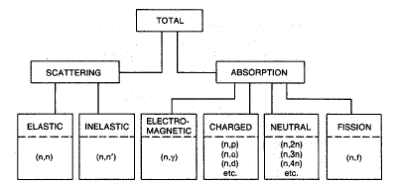
\includegraphics[scale=0.7]{ch5/image1}
	\captionof{figure}{ }
	\end{wrapfigure}
Il existe deux principaux types d'interactions
\begin{enumerate}
\item[$\bullet$] \textit{Diffusion} : l'énergie et la trajectoire du neutron est modifiée mais le 
noyau conserve un nombre de nucléons identique
\item[$\bullet$] \textit{Absorption} : modification du noyau cible causant l'émission de rayonnements.
\end{enumerate}

\subsection{Diffusion élastique $(n,n)$}%sl8
Durant une \textbf{collision élastique}, l'énergie cinétique totale du neutron et du noyau est 
inchangée : le noyau cible ($m_2$) au repos reçoit du neutron ($m_n,E$) une énergie cinétique
$T_c$ comprise entre 0 et 
\begin{equation}
T_{max}=\frac{4m_nm_2}{(m_n+m_2)^2}E
\end{equation}
Un neutron peut communiquer toute son énergie à un atome d'hydrogène. La diffusion élastique est
alors très efficace pour ralentir des neutrons si $m_2\approx m_n$.\\

Introduisons l'angle de recul $\theta_r$ du noyau. Celui-ci peut être lié à l'énergie transférée
$T_c$ par conservation de l'énergie et de l'impulsion
\begin{equation}
T_{c}=\frac{4m_nm_2}{(m_n+m_2)^2}E\cos^2\theta_r = \frac{4\alpha}{(\alpha+1)^2}E\cos^2\theta_r
\end{equation}
où $\alpha = m_2/m_n$. Il est dès lors nécessaire de déterminer la section efficace différentielle
angulaire pour connaître l'énergie cédée par le neutron. Pour se faire, il faut distinguer les 
deux types de collision élastique
\begin{enumerate}
\item Interaction directe avec le noyau. A faible énergie, la section efficace tend vers $4\pi R^2$ 
(ordre d'un barn).
\item En deux temps. Premièrement formation d'un noyau dans un état excité. Secondement, émission d'un 
neutron pour former l'atome de départ.La section efficace dépend donc de l'énergie du neutron et 
le noyau excité ne peut être formé que dans des états bien définis
\end{enumerate}\ \\


	\begin{wrapfigure}[11]{l}{6.5cm}
	\vspace{-5mm}
	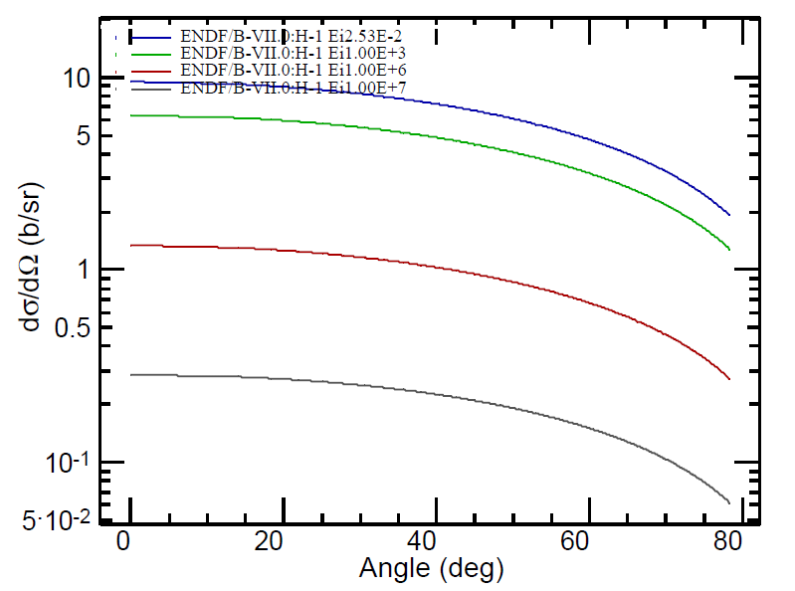
\includegraphics[scale=0.3]{ch5/image2}
	\captionof{figure}{ }
	\end{wrapfigure}
	
La section efficace totale n'est pas simplement la somme des deux effets à cause des interférences. 
On va ici s'intéresser au cas le plus simple où $\alpha=1$ : la distribution angulaire varie alors
en $\cos\theta_r$ (la distribution angulaire de $\theta_n$ correspond à celle de $\theta_r$).\\

On a donc comme valeur moyenne de l'énergie transférée $\langle T_c\rangle \propto \langle
\cos^2\theta_r\rangle = 1/2$
\begin{equation}
\langle T_c \rangle =\frac{2\alpha}{(\alpha+1)^2}E
\end{equation}
Il s'agit bien entendu d'une grosse approximation mais le résultat est tout de même correct. Ainsi, 
pour de l'hydrogène ($\alpha=1$) $\langle T_c \rangle = E/2$. De manière générale, l'énergie du 
neutron $E^{'(n)}$ après $n$ collisions élastiques vaut
\begin{equation}
\langle E'^{(n)} \rangle =\left[\frac{(\alpha^2+1)}{(\alpha+1)^2}\right]^nE
\end{equation}
Pour atteindre une énergie $E^{'(n)}$ à partir d'une énergie $E$, il faut que le neutron subissent
en moyenne $n$ collisions élastiques avec\footnote{Voir cours \textit{Nuclear Reactor Physics}})
\begin{equation}
n = \frac{\log{(E'^{(n)}/E)}}{\log{[(A^2+1)/(A+1)^2]}}
\end{equation}
Après un choc élastique dû à un neutron rapide, le noyau est déplacé et - s'il possède une énergie
cinétique suffisante - peut déplacer d'autres noyaux. Il en résulte une cascade de déplacements
atomiques dans un volume de rayon de 100 $\AA$. Pour que ce soit possible, il faut avoir une 
certaine \textit{énergie de seuil de déplacement} de l'ordre de 25 eV.

\subsection{Diffusion inélastique $(n,n')$}%sl15
Le noyau cible est maintenant amené dans un état excité et l'énergie du neutron est convertie sous
la forme d'énergie cinétique et potentielle du noyau cible. Pour se faire, cette réaction passe
par la formation d'un noyau composé avec ensuite émission d'un neutron pour reformer le noyau dans
un état excité qui, souvent, retourne dans son état fondamental par émission de $\gamma$. \\

Pour se produite, l'énergie cinétique du neutron doit dépasser un certain seuil
\begin{equation}
E_{seuil}=\frac{A+1}{A}E_{exc}
\end{equation}
où $E_{exc}$ est l'énergie d'excitation du noyau. 


\subsection{Absorption}%sl17
Après une absorption, un rayonnement secondaire peut être émis et détecté. Celui-ci peut être
\begin{itemize}
\item[$\bullet$] Un rayonnement $\gamma \to (n,\gamma)$
\item[$\bullet$] Une particule chargée $(p,\alpha)\to (n,p)$ ou $(n,
\alpha)$.
\item[$\bullet$] Des neutrons $(n,2n), (n,3n),\dots$
\item[$\bullet$] Des produits de fission $(n,f)$
\end{itemize}

\subsubsection{Absorption électromagnétique}
La capture radiative est une réaction $(n,\gamma)$ où le neutron est absorbé par le noyau pour former
un noyau dans un état excité qui émet un ou plusieurs $\gamma$. Celle-ci présente des résonances et 
domine surtout aux faibles énergies.

\subsubsection{Absorption suivie de l'émission de particules chargées}
Il s'agit souvent de l'émission d'un proton $(n,p)$ ou d'un $\alpha$ $(n,\alpha)$. Ces réactions
se produisent souvent avec des neutrons rapides car étant endoénergétique, il faut apporter une 
certaine énergie (pour franchir la barrière de potentiel du noyau).

\subsubsection{Absorption suivie d'une réaction de fission}
Se produit pour des matériaux à $Z$ élevé quand la capture d'un neutron conduit à la scission du noyau et à la production de fragments lourds ainsi que de nucléons de grande énergie cinétique. Ceci est
vu en long et en large dans le cours traitant des réacteurs nucléaires, je ne m'attarde pas la dessus
ici.

\section{Sections efficaces d'interaction}%sl21
La section efficace totale est la somme des sections efficaces des différents processus mais il 
n'existe pas de calculs complets de section efficace : il faut mélanger les résultats théoriques
et expérimentaux. De façon générale (tendance, pas une règle) la section efficace totale diminue 
lorsque l'énergie du neutron augmente. La section efficace de diffusion élastique est 
approximativement constante et celle d'absorption varie en $1/v$. La section efficace totale est
donc soit constante, soit varie en $1/v$ selon le processus dominant. Pour les matériaux à $Z$
élevé, les nombreuses résonances des réactions de fissions peuvent dominer la loi en $1/v$.\\

Les slides 23 a 28 donnent des exemples de section efficaces. Considérons la transmission d'un
faisceau de neutrons à travers une cible épaisse comme nous l'avions fait pour les photons\footnote{
A cause du phénomène de multiplication et la diffusion multiple, cette équation est souvent fausse.}
\begin{equation}
I=I_0\exp{(-N\sigma_tx)}
\end{equation}
On définit alors la \textbf{section efficace macroscopique} (m$^{-1}$) telle que
\begin{equation}
\Sigma_t=N\sigma_t
\end{equation}

\section{Modération et parcours des neutrons} %sl30
Deux facteurs sont important pour ralentir un neutron rapide
\begin{enumerate}
\item La probabilité de diffusion
\item La modification de son énergie moyenne
\end{enumerate}
On définit alors le pouvoir de modération comme
\begin{equation}
MP=\xi\Sigma_s
\end{equation}
où $\xi$ est le décrément logarithmique moyen en énergie et $\Sigma_s$ la section efficace 
macroscopique de scattering.

\subsection{Rapport de modération}
Ralentir c'est bien, mais si tout est absorbé ça ne sert pas à grand chose ! Il faut que 
l'absorption soit faible et on défini pour ça un \textbf{pouvoir de modération} (\danger)
\begin{equation}
MR=\frac{\xi\Sigma_s}{\Sigma_a}
\end{equation}
où $\Sigma_a$ est la section efficace macroscopique d'absorption.\\

Pour modérer les neutrons rapide on utilise donc bien des matériaux qui ont une masse proche
de celle du neutron et bien évidemment \textbf{pas} du plomb.